
\section{Results}
% % 4 most important figures: heatmap OECD, heatmap support, prioritization or conjoint (r), list exp (table)
\subsection{Data}
%\textcolor{red}{\textbf{Beware, data collection is still ongoing (we have 80\% of the final sample) so results are partial and not definitive. Please do not cite at this stage.}} \\ 
Stated support for different global policies has been measured in % TD better way to sell these results?
a survey on climate attitudes conducted in 2021 on 40,680 respondents from 20 countries covering 72\% of global CO$_\text{2}$ emissions (the questions of this survey on national policies are analysed in another paper: \citealp{dechezlepretre_fighting_2022}). We conduct complementary surveys in the U.S. and four European countries to study in detail the sincerity and rationales behind the support for the GCS, the attitudes toward various global policies, global redistribution, and universalistic values. The U.S. survey has been divided in two waves: \textit{US1} and \textit{US2}, with respectively 3,000 and 2,000 respondents. The European survey, called \textit{Eu}, combines the two U.S. waves (just without one question of US2 that uses results from US1). The Eu survey comprises 3,000 respondents representative of France, Germany, Spain and the UK, along the dimensions of gender, income, age, highest diploma, country, and degree of urbanisation. The U.S. samples are representative along the same dimensions (with \textit{region} instead of \textit{country}) as well as along ethnicity. Tables \ref{tab:representativeness_waves}-\ref{tab:representativeness_EU} confirm that our samples closely match population frequencies. The questionnaires are given in Appendices \ref{app:questionnaire_oecd} and \ref{app:questionnaire}.

\begin{table}[h]\label{tab:surveys}
  \caption[Surveys summary]{Characteristics of the different surveys.} 
  \centering
\begin{tabular}
  {@{\extracolsep{5pt}}lcccc} 
  \\[-1.8ex]\hline 
  \hline \\[-1.8ex] 
  \\[-1.8ex] Survey & Global & Eu & US1 & US2 \\ 
  \hline \\[-1.8ex]   
  Country coverage & 20 countries & FR, DE, ES, UK & U.S. & U.S. \\ 
  Sample size & 40,680 & 3,000 & 3,000 & 2,000 \\ 
  % Median duration (in min) & 28 & 20 & 14 & 11 \\ 
  % Date of administration & 03/21--03/22 & 02--03/23 & 01--03/23 & 03--04/23 \\ 
  \hline 
  \hline \\[-1.8ex] 
\end{tabular}
\end{table}

\subsection{International support}
The global survey shows strong support for climate policies enacted at the global level (Figure \ref{fig:oecd}). When asked ``At which level(s) do you think public policies to tackle climate change need to be put in place?'', 70\% (in the U.S.) to 94\% (in Japan) choose the global level. Meanwhile, the European level is chosen by less than half of the European respondents while the federal level is chosen by only 52\% of U.S. respondents. More local levels are generally chosen less than broader ones. This preference for the global level is in line with \citet{beiser-mcgrath_could_2019} and consistent with (at least) two of the three key motives for supporting climate policies identified in the literature %:
\citep{klenert_making_2018,douenne_yellow_2022,dechezlepretre_fighting_2022}: effectiveness and fairness (the third being self-interest). % GCS more supported in Eu than global T&D. Possible explanations: quota vs. tax, climate club, better understanding / survey fatigue

\begin{figure} % TD have a simpler title (e.g. "Attitudes towards global climate policies"), and a note explaining what the figure exactly does (unit of the numbers, meaning of the colors, exclusion of indifferent people, etc.
  % MAJOR figure
  \caption[Relative support for global climate policies]{Relative support for global climate policies. \\ Share of \textit{Somewhat} or \textit{Strongly support} among non-\textit{indifferent} answers (in percent, $n$ = 40,680). The color blue denotes a relative majority. See Figure \ref{fig:oecd_absolute} for the absolute support. (Questions \ref{q:scale}-\ref{q:millionaire_tax})} 
  \makebox[\textwidth][c]{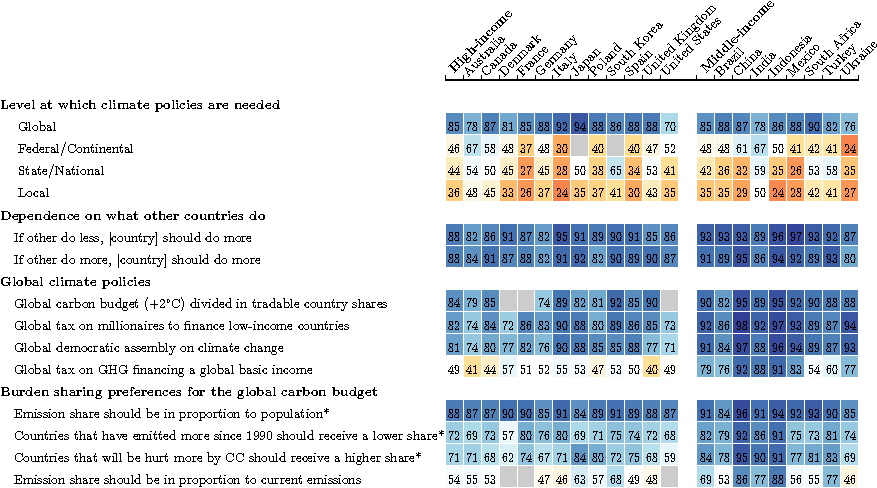
\includegraphics[width=1.2\textwidth]{../figures/OECD/Heatplot_burden_share_all_share_countries.pdf}}\label{fig:oecd}
  {\footnotesize *In Denmark, France and the U.S., the questions with an asterisk were asked differently, cf. Question \ref{q:burden_sharing_asterisk}. } 
\end{figure}

Several global policies obtain an absolute majority (i.e. \textit{somewhat} or \textit{strong}) %more than 70\% relative %
support in all countries: %a tax on millionaires to finance low-income countries, a consultative assembly on climate change, and a global quota on CO$_\text{2}$ emissions divided in tradable country shares.\footnote{These policies are respectively described as follows: 
``a tax on all millionaires in dollars around the world to finance low-income countries that comply with international standards regarding climate action [which] would finance infrastructure and public services such as access to drinking water, healthcare, and education'', ``a global democratic assembly whose role would be to draft international treaties against climate change [where] each adult across the world would have one vote to elect members of the assembly'' (though this one receives only 48\% of support in the U.S.), % we haven't yet defined absolute support at this stage
and an international emissions trading system where ``countries that emit more than their national share would pay a fee to countries that emit less than their share''. 
%} 
In high-income countries, this global quota obtains 64\% of absolute %(i.e. \textit{somewhat} or \textit{strong}) 
support and 84\% of relative support (i.e. excluding \textit{indifferent} answers). The support is even higher in middle-income countries, though one should interpret the results with caution in middle-income countries as their samples are only representative of the online population (young, graduated and urban people are over-represented). 

After the support for the global quota, respondents are asked how the carbon budget should be divided among countries. 
Consistent with the literature (see Appendix \ref{subsubsec:literature_attitudes_burden_sharing}), the preferred burden-sharing rule is to allocate the rights to emit on an equal per capita basis: this fairness principle secures an absolute majority support in all countries, and a relative majority support never below 84\%. 
Taking into account historical responsibilities or vulnerability to climate damages is also popular, though less consensual, while grand-fathering (i.e. allocating emission shares in proportion to current emissions) comes last everywhere. 

The Global Climate Scheme, i.e. a global quota where emission rights are allocated on an equal per capita basis, has the same distributive effects as a global carbon tax that would fund a global basic income. The support for the latter policy is also tested, and there the redistributive effects are specified to the respondents (the average increase in expenditures along with the amount of the basic income, see the box below). %: the \$30 per month basic income would lift the 700 million people who earn less than \$2/day out of extreme poverty, and fossil price increases would cost the typical person in their country a certain amount (that is provided).  % The average British person would lose a bit from this policy as they would face £42 per month in price increases, which is higher that the £22 they would receive.
The levels of support are consistent with the findings of \citet{carattini_how_2019}, the only previous study that tested a global carbon tax. Despite their similarity, the global tax is less supported than the global quota, and it even fails to obtain a relative majority in Anglo-saxon countries. This lower support is likely due to the facts that distributive effects are made salient in the case of the tax, and that people may find a quota more effective than a tax to reduce emissions. This interpretation is consistent with the level of support for the global quota once we make the distributive effects salient, which we do in the complementary surveys. % though we cannot exclude that people find a quota more effective than a tax to reduce emissions. 


\subsection{Stated support for various policies}
% H0: Majority support for each global policies except maximum wealth and debt cancellation
The remainder of the paper analyzes the results from the complementary surveys in the U.S. and in Europe. This Section covers the stated support for different global redistributive policies. %the Global Climate Scheme, a global wealth tax, other global policies, and foreign aid.

\subsubsection{Global Climate Scheme} % NCCcomment
In the complementary surveys, we describe the Global Climate Scheme, explain its distributive effects (specifying the amounts at stake, cf. the box below), %Appendix \ref{app:gain_gcs}), 
test the understanding that typical people would lose in high-income countries and that the poorest humans would win using an incentivized question, and then give the correct answer. We proceed the same way for a National Redistribution Scheme (NR) that would tax the top 5\% (in the U.S.) or the top 1\% (in Europe) to finance cash transfers to all adults (calibrated to offset the monetary loss of the GCS for the median emitter), expecting people to find out at the comprehension question that the richest would lose and the typical people in their country would win. Then, we summarize both schemes to make sure that the respondents remember them. Right after, we ask a last incentivized question of comprehension, and later give the expected answer that a typical fellow citizen would neither win nor lose with the GCS and NR combined. Finally, we directly ask the support for the GCS and for NR in a simple \textit{Yes}/\textit{No} question. The stated support for the GCS is at 54\% in the U.S. and 76\% in Europe, and the support for NR is very close, at 56 and 73\%, respectively (Figure \ref{fig:support_binary}). % TD add something if equality remains
Appendix \ref{app:determinants} presents the sociodemographic determinants of the support for the GCS, and shows e.g. a stronger support among young people. %\ref{tab:gcs_determinant} 

\begin{figure}[h!]
    \caption[Support for the Global Climate Scheme]{Support for the GCS, NR and the combination of GCS, NR and C. (Questions \ref{q:gcs_support}, \ref{q:nr_support} and \ref{q:crg_support}).%; $n_\text{US} = n_\text{Eu} = 3,000,\, n_\text{FR} = 729,\, n_\text{DE} = 929,\, n_\text{ES} = 543,\, n_\text{UK} = 749$)
    }\label{fig:support_binary}
    \makebox[\textwidth][c]{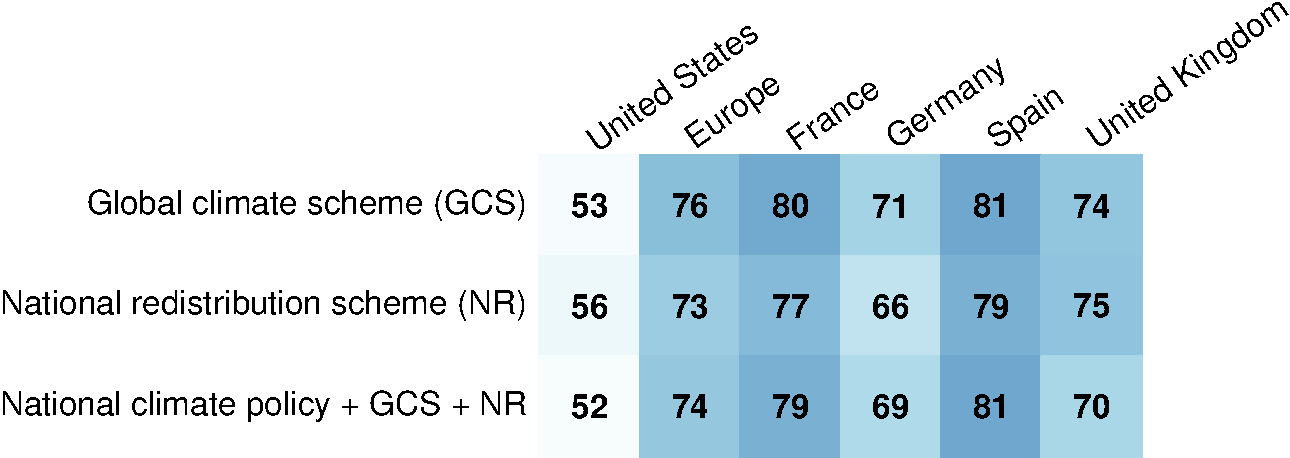
\includegraphics[width=.9\textwidth]{../figures/country_comparison/support_binary_positive.pdf}} 
\end{figure}

\begin{tcolorbox}
  \paragraph{The Global Climate Scheme} The GCS consists of a global cap-and-trade system, where emission rights are auctioned each year to polluting firms, and of a global basic income, funded by the auction revenues. 
  % I have added the following lines. TODO? put in a footnote?
  Using the price and emissions trajectories from the report by \cite{stern_report_2017}, %Stern-Stiglitz report,\cite{stern_report_2017} 
  and in particular a carbon price of \$90/tCO$_\text{2}$ in 2030, we estimate that the basic income would amount to \$30 per month for each human above 15 (see details in Appendix \ref{app:gain_gcs}). %, enough to lift out of extreme poverty the 700 million people who live with less than PPP \$2 per day. Conversely, assuming a carbon price of \$90/tCO$_\text{2}$ in 2030, high emitters like a typical American (with median U.S. CO$_\text{2}$ emissions) would lose in net \$85 per month, as they would face \$115 per month in price increases (see details in Appendix \ref{app:gain_gcs}). 
  When describing the GCS to the respondents, we specify its redistributive effects. Namely, %the \$30 per month basic income would lift 
  the 700 million people with less than \$2/day would be lifted out of extreme poverty, and fossil price increases would cost the typical person in their country a specified amount, despite the basic income (see the exact wording in Appendix \ref{subsec:questionnaire_GCS}). This median net cost is \$85 in the U.S., \euro{}10 in France, \euro{}25 in Germany, \euro{}5 in Spain, £20 in the UK. % . We specify the net monthly cost for the median emitter of the country
\end{tcolorbox}

\subsubsection{Global wealth tax} 
Consistent with the global survey's results, a ``tax on millionaires of all countries to finance low-income countries'' receives an absolute majority support of more than 67\% in every country, only 5 p.p. lower than a national millionaires tax overall (Figure \ref{fig:support}). % us2!
To random subsamples, we ask respondents how the revenues of a global tax on individual wealth in excess of \$5 million should be shared with low-income countries, after describing how much revenues such a tax would raise in their country vs. in low-income countries.\footnote{Namely, a 2\% tax on net wealth above \$5 million would raise each year \euro{}5 billion in Spain, \euro{}16 billion in France, £20 billion in the UK, \euro{}44 billion in Germany, \$430 billion in the U.S., and \$1 billion in all low-income countries taken together (28 countries, home to 700 million people).} To some respondents ($n$ = 891), we ask what percentage of the global tax revenues should be pooled to finance low-income countries. In each country, at least 88\% of respondents answer a positive amount, with an overall average of 30\% (Germany) to 36\% (U.S., France) (Figure \ref{fig:global_share_mean}). To some other respondents ($n$ = 859), we ask whether they would prefer that each country retains the revenues it collected or that half of the revenues be pooled to finance low-income countries. About half of the people prefer to channel half of the tax revenues to low-income countries. 

\begin{figure}
    \centering 
    \caption[Preferred share of wealth tax for low-income countries]{Percent of global wealth tax that should finance low-income countries (\textit{mean}). (Question \ref{q:global_tax_global_share})} % TODO! n
    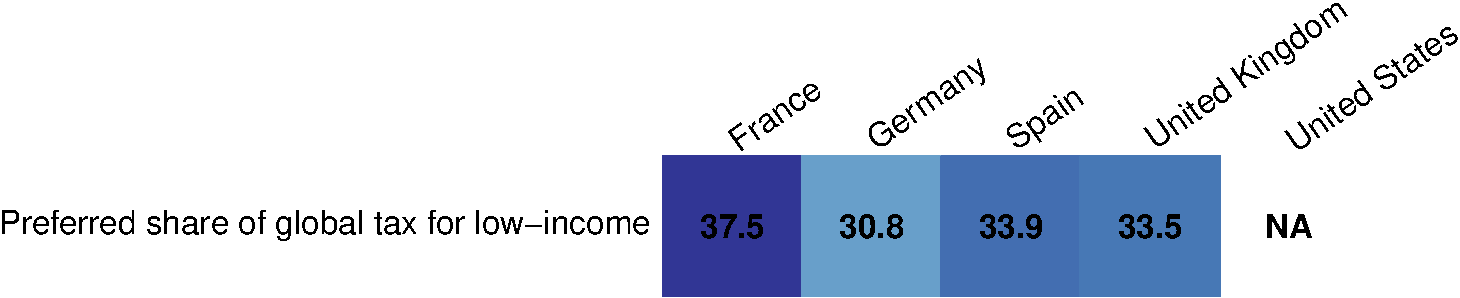
\includegraphics[width=1\textwidth]{../figures/country_comparison/global_tax_global_share_mean.pdf} \label{fig:global_share_mean}
\end{figure}

\subsubsection{Other global policies} % NCCcomment
We also test support for other %more realistic
global policies (Figure \ref{fig:support}). All receive relative majority support in each country except two:  the ``cancellation of low-income countries' public debt'' and ``a maximum wealth limit'' (the latter obtains relative majority support in Europe but not in the U.S., despite the cap being defined as \$10 billion the U.S. instead of \euro{}/£100 million in Europe). Climate-related policies are particularly popular: ``high-income countries funding renewable energy in low-income countries'' obtains absolute majority support everywhere while loss and damages compensation (which was approved at the COP27) receives a relative support of 55\% (U.S.) to 81\% (Spain).

\begin{figure}
  % MAJOR figure
  \caption[Relative support for various global policies]{Relative support for various global policies (percentage of \textit{somewhat} or \textit{strong support}, after excluding \textit{indifferent} answers). (Questions \ref{q:climate_policies} and \ref{q:other_policies}; See Figure \ref{fig:support_likert_positive} for the absolute support.)% $n_\text{US} = n_\text{Eu} = 3,000,\, n_\text{FR} = 729,\, n_\text{DE} = 929,\, n_\text{ES} = 543,\, n_\text{UK} = 749, n_\text{US, global/national wealth tax} = 2,000$
  } % ; $n$ = 6,000
  \makebox[\textwidth][c]{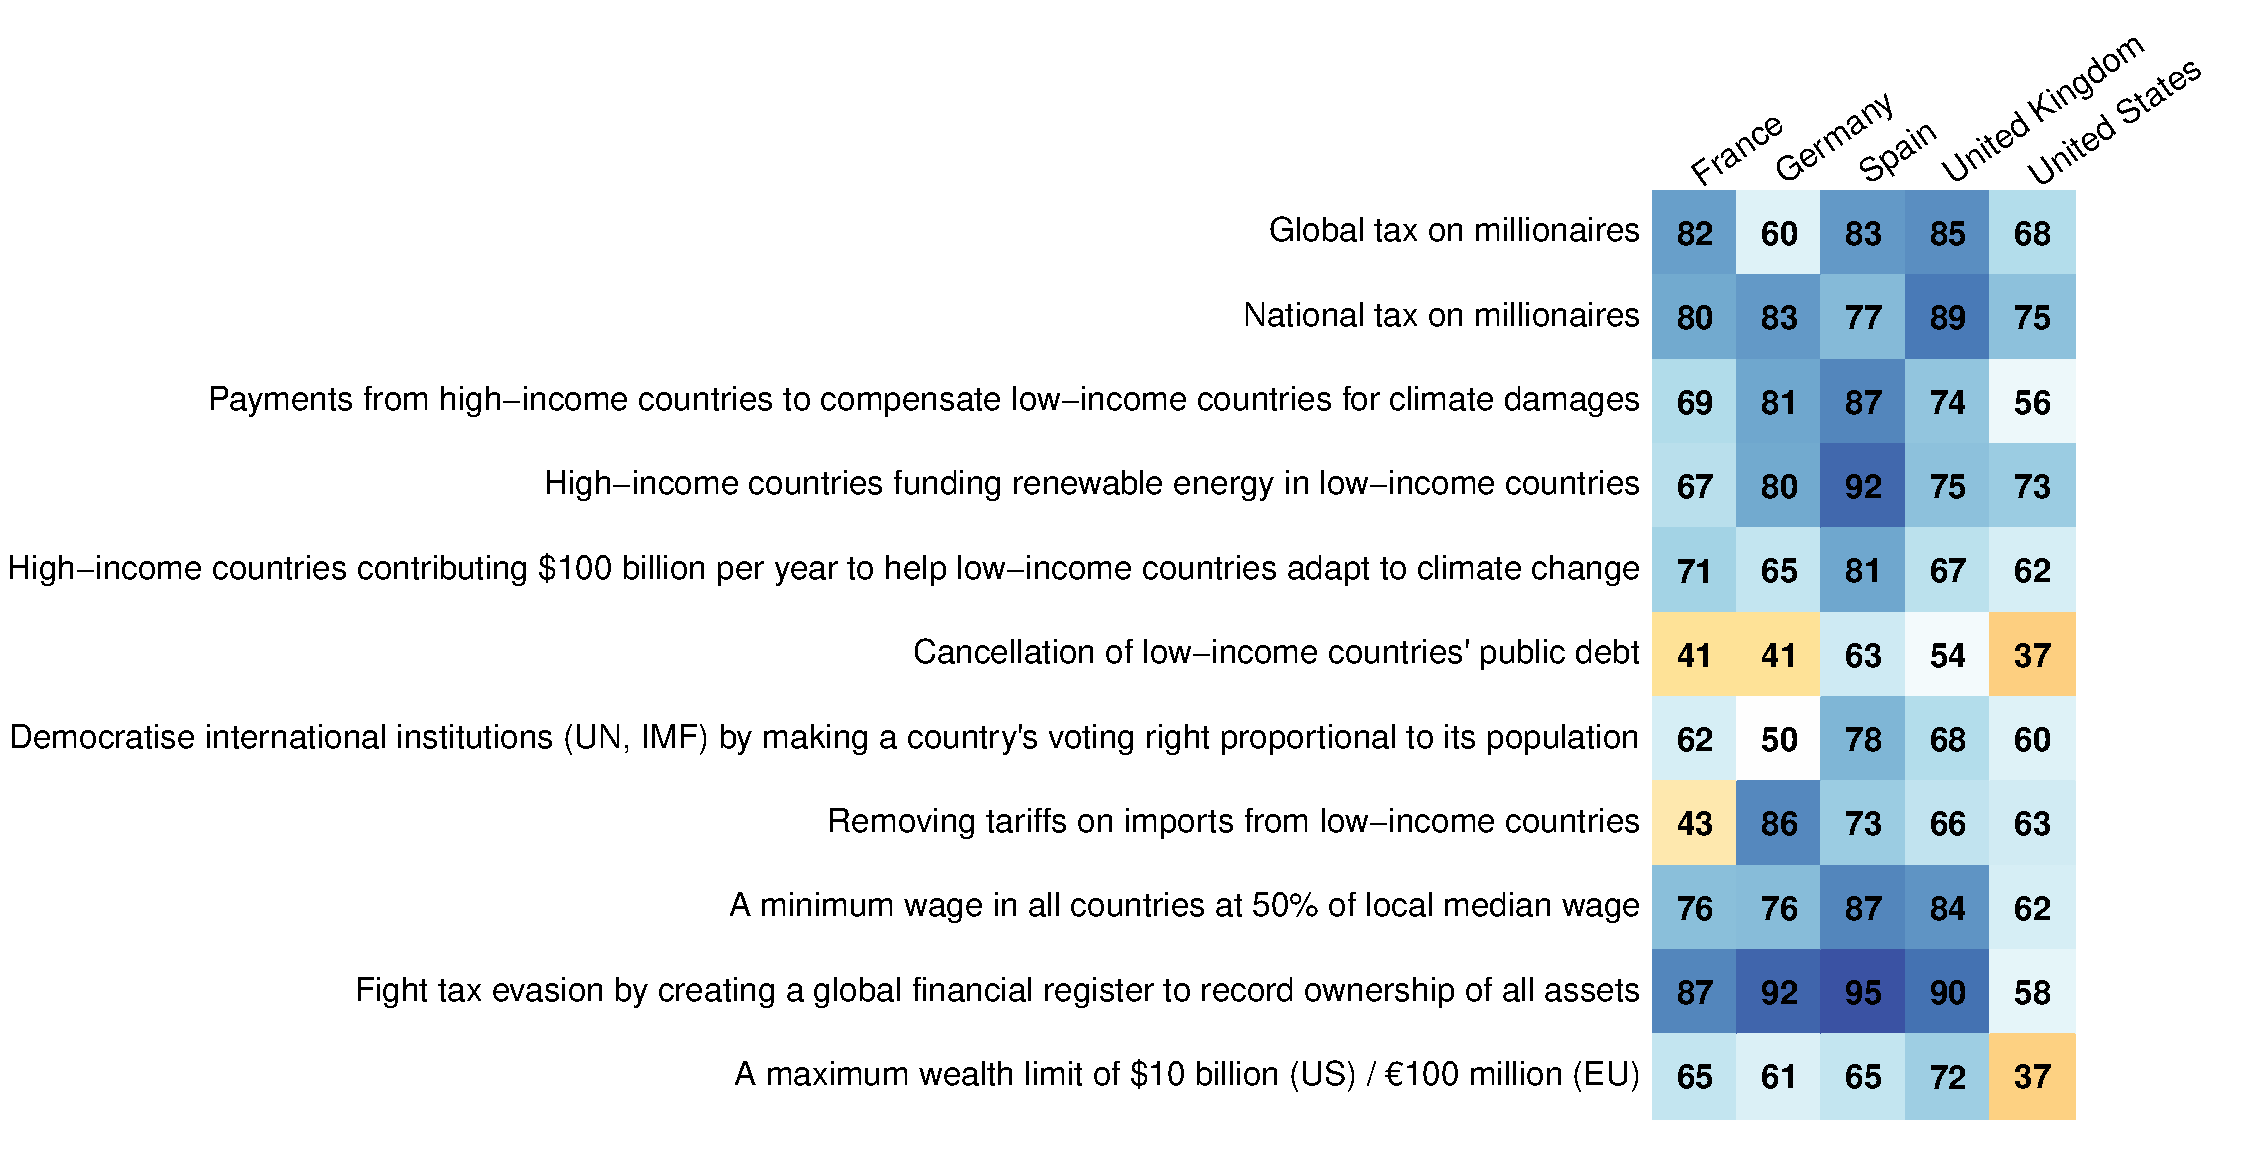
\includegraphics[width=\textwidth]{../figures/country_comparison/support_likert_share.pdf}}\label{fig:support}
\end{figure} 

% H0: Foreign aid: less than 20\% want a decrease (because nationalist), median wants increase at some conditions (no diversion, human rights) => GCS mostly addresses these points
\subsubsection{Foreign aid} % NCCcomment
%eu! 
After providing the amount %explaining that ``0.4\% of U.S. government spending (that is, 0.2\% of U.S. GDP) is 
``spent on foreign aid to reduce poverty in low-income countries'' (in proportion to their country's government spending and GDP), less than 16\% state that their country's foreign aid should be reduced while 62\% state that it should be increased, including 17\% who support an unconditional increase (Figure \ref{fig:foreign_aid_raise_support}). To the 45\% who answer that aid should be increased but only if some conditions are respected, we later ask them what condition(s) should be required (Figure \ref{fig:foreign_aid_condition}). The three conditions most chosen are largely respected by the Global Climate Scheme: % TODO? nuance more? I have changed from "all largely respected"
``that we can be sure the aid reaches people in need and money is not diverted'' (chosen by 73\%), ``that recipient countries comply with climate targets and human rights'' (67\%), and ``that other high-income countries also increase their foreign aid'' (48\%). %, we propose different conditions. The most chosen condition (by 74\%) is  and the second most (by 59\%) ``That recipient countries comply with climate targets and human rights''. 
On the other side, not wishing to increase their country's foreign aid is mostly justified by prioritizing one's fellow citizens or viewing each country as responsible for its own fate (Figure \ref{fig:foreign_aid_no}). In an open-ended question asking what high-income countries should do to fight extreme poverty, a large majority of Americans expressed that more help is needed (Figure \ref{fig:poverty_field}). The most cited form of aid proposed is monetary, followed by investments in education.

\begin{figure}[h!]
  \caption[Attitudes on the evolution of foreign aid]{Attitudes regarding the evolution of [own country] foreign aid. (Question \ref{q:foreign_aid_raise_support})}\label{fig:foreign_aid_raise_support}
  \makebox[\textwidth][c]{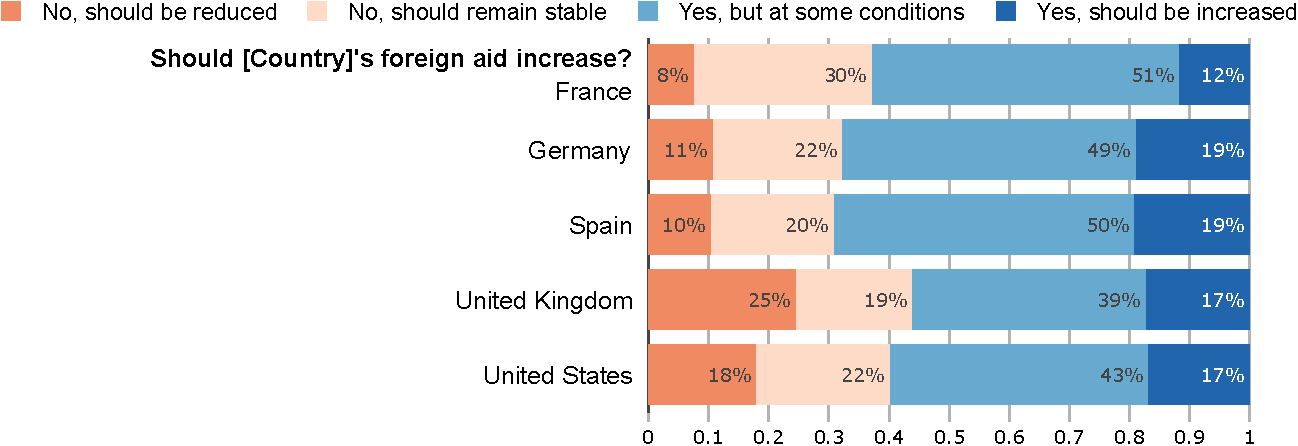
\includegraphics[width=\textwidth]{../figures/country_comparison/foreign_aid_raise_support.pdf}} 
\end{figure}

\begin{figure}[h!]
  \caption[Conditions at which foreign aid should be increased]{Conditions at which foreign aid should be increased (in percent). [Asked to those who wish an increase of foreign aid at some conditions.] (Question \ref{q:foreign_aid_condition})}\label{fig:foreign_aid_condition}
  \makebox[\textwidth][c]{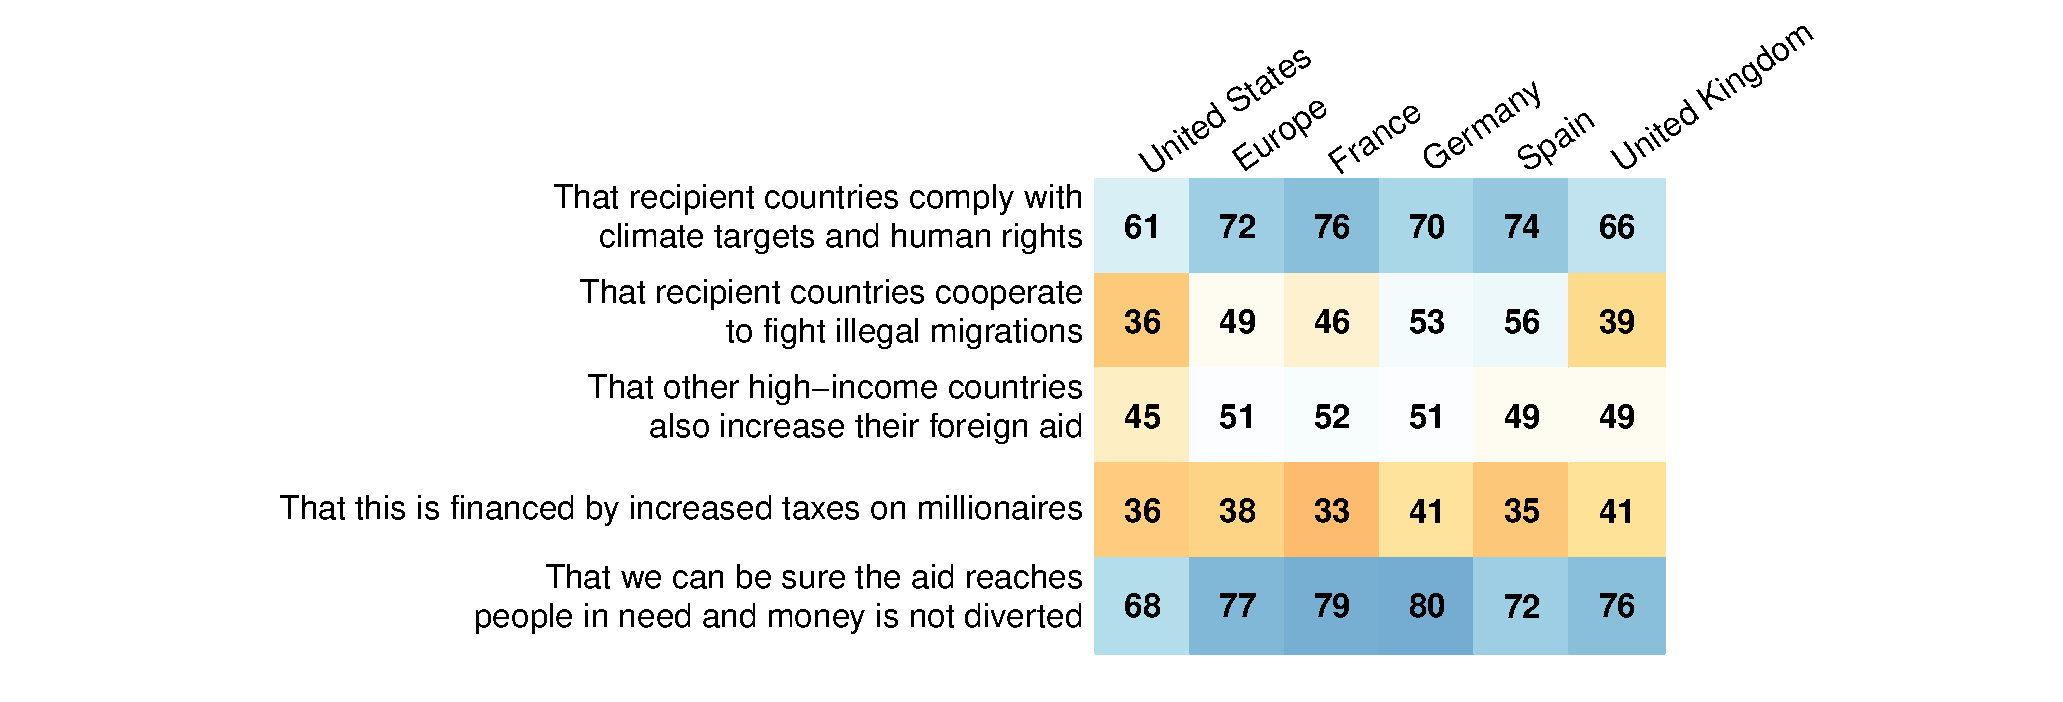
\includegraphics[width=\textwidth]{../figures/country_comparison/foreign_aid_condition_positive.pdf}} 
\end{figure}

\begin{figure}[h!]
  \caption[Reasons why foreign aid should not be increased]{Reasons why foreign aid should not be increased (in percent). [Asked to those who wish a decrease or stability of foreign aid.] (Question \ref{q:foreign_aid_no})}\label{fig:foreign_aid_no}
  \makebox[\textwidth][c]{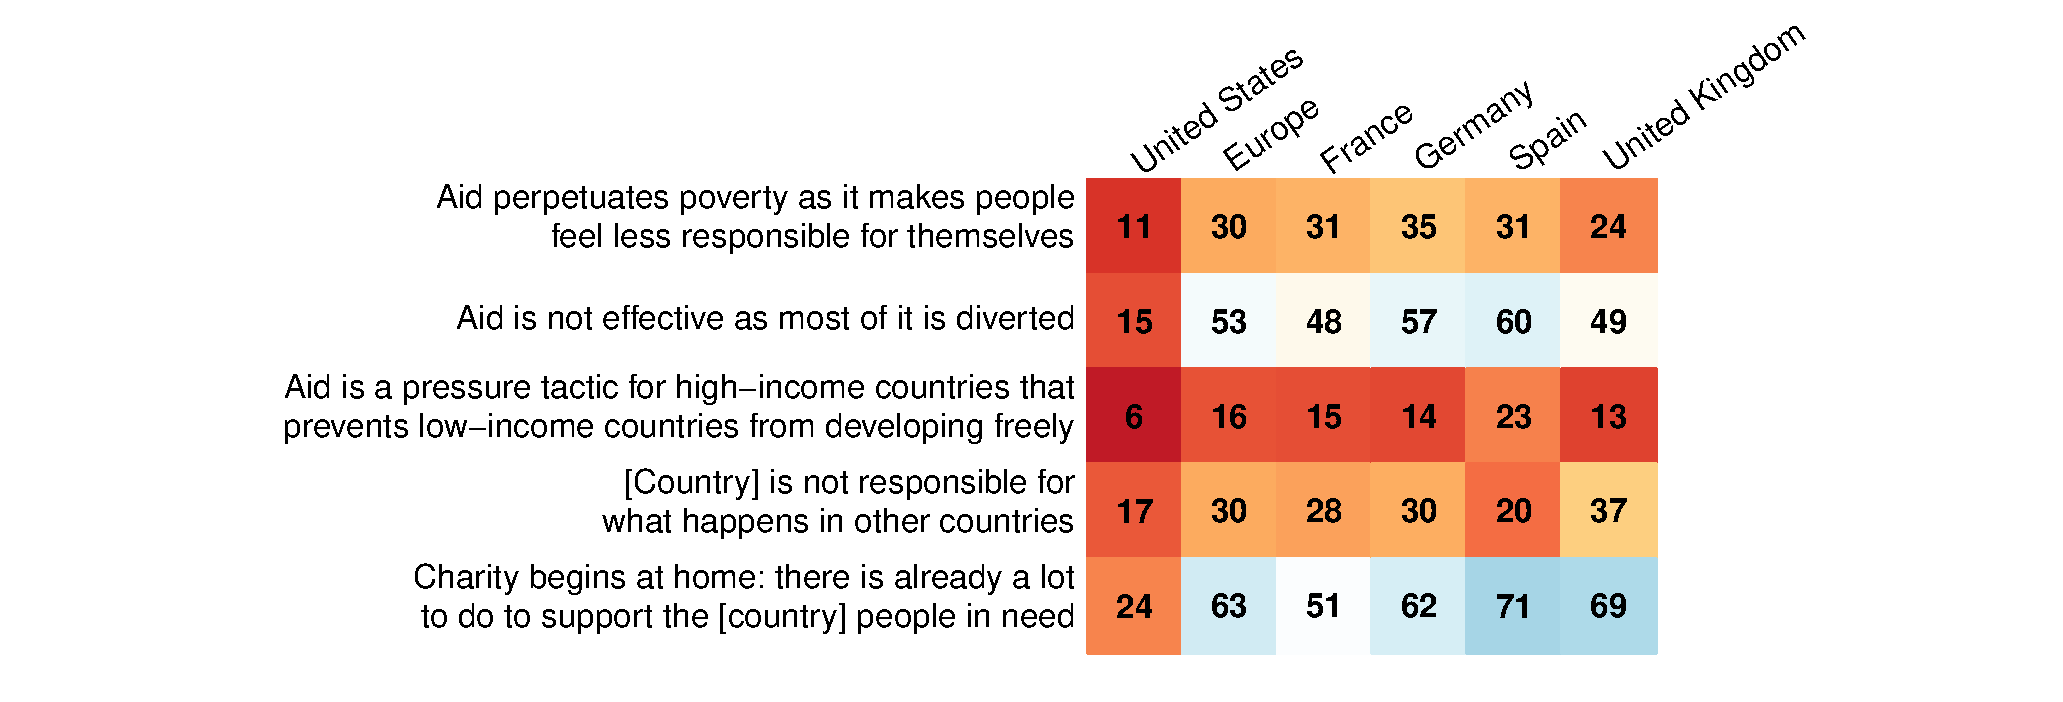
\includegraphics[width=\textwidth]{../figures/country_comparison/foreign_aid_no_positive.pdf}} 
\end{figure}

\subsection{Sincerity of support}

We use several methods to assess the sincerity of the support for the Global Climate Scheme: a list experiment, a real-stake petition, conjoint analyses, and the prioritization of policies. All methods suggest that the support is either completely sincere, or the share of insincere answers is limited. 

\subsubsection{List experiment}\label{subsubsec:list_exp}  % NCCcomment
% H1: List experiment: There seems to be a 8pp social norm (differential of 3pp with NR). No effect of the number of options. TODO: check literature

By asking \textit{how many} policies within a list respondents support and varying the list among respondents, a list experiment allows identifying the tacit support for a policy of interest. The tacit support is estimated as the difference in the average number of policies supported between two groups, whose list differ only by the inclusion (or not) of that policy \citep{hainmueller_causal_2014}. % respondents who face a list containing the policy, and respondents who face the same list without it. 
List experiments have been used to reveal a social desirability bias that silences either racism in Southern U.S. \citep{kuklinski_racial_1997} or the opposition to the invasion of Ukraine in Russia \citep{chapkovski_solid_2022}. % TODO? remove?
As shown in Table \ref{tab:list_exp}, the tacit support for the GCS measured through the list experiment is not significantly lower than the direct stated support.\footnote{We use the difference-in-means estimator. The confidence intervals are computed through Monte Carlo simulation using the R package \textit{list} (see \citealp{imai_multivariate_2011}).} Thus, we cannot reject an absence of social desirability bias in our case.
% The tacit support for the GCS measured through the list experiment is as high as  the direct question in Eu but significantly lower by 5 p.p. in the U.S. This may be the sign of a social norm pushing some Americans to state that they support the GCS although they secretly do not. Still, if there is a social norm in favor of the GCS, there is a similar norm in favor of the National Redistribution Scheme, as the gap between the tacit and direct support for it is comparable (at 6 p.p.). %However, two observations qualify this interpretation. First, the gap between the tacit and direct support for the National Redistribution Scheme is comparable (at 7 p.p.) though we did not expect such a social norm in the case of the national redistribution, as the 95\% who would benefit from it should not feel ashamed to oppose a policy that would benefit them. Second, while we tested the questionnaire on random people in cafés, we noticed that some were confused by the question of the list experiment (asking how many policies from the list they supported), upset with the conservative societal policy (``Marriage only for opposite-sex couples in the U.S.'', ``Death penalty for major crimes'' in Europe), to the point that they did not answer attentively.

\begin{table}[h]
  % MAJOR figure % TODO! same table for NR in appendix
  % TODO table by country
  \caption[List experiment: tacit support for the GCS]{Number of supported policies in the list experiment depending on the presence of the Global Climate Scheme (GCS) in the list.%in function of the composition of the list. GCS stands for the Global Climate Scheme and NR for the National Redistribution Scheme.} % Beware, this question is quite unusual. \\ Among the policies below, how many do you support?  \\ Coal exit, Marriage only for opposite-sex couples 
  }\label{tab:list_exp}
  \makebox[\textwidth][c]{
\begin{tabular}{@{\extracolsep{5pt}}lccc} 
\\[-1.8ex]\hline 
\hline \\[-1.8ex] 
 & \multicolumn{3}{c}{Number of supported policies} \\ 
\cline{2-4} 
\\[-1.8ex] & All & US & Europe \\ 
\hline \\[-1.8ex] 
 List contains: GCS & 0.624$^{***}$ & 0.524$^{***}$ & 0.724$^{***}$ \\ 
  & (0.028) & (0.041) & (0.036) \\ 
\hline  \\[-1.8ex] \textit{Support for GCS} & 0.65  &  0.542  &  0.757 \\
\textit{Social desirability bias} & \textit{$ -0.026 $} & \textit{$ -0.018 $} & \textit{$ -0.033 $}\\
\textit{80\% C.I. for the bias} & \textit{ $[ -0.06 ; 0.01 ]$ } & \textit{ $[ -0.07 ; 0.01 ]$} & \textit{ $[ -0.08 ; 0.01 ]$}\\
 \hline \\[-1.8ex] 
Constant & 1.317 & 1.147 & 1.486 \\ 
Observations & 6,000 & 3,000 & 3,000 \\ 
R$^{2}$ & 0.089 & 0.065 & 0.125 \\ 
\hline 
\hline \\[-1.8ex] 
\textit{Note:}  & \multicolumn{3}{r}{$^{*}$p$<$0.1; $^{**}$p$<$0.05; $^{***}$p$<$0.01} \\ 
\end{tabular} 
  }
  % {\footnotesize \textit{Note:} $^{*}p<0.1$; $^{**} p<0.05$; $^{***} p<0.01$.}
\end{table}

% Donation addresses experimenter demand
\subsubsection{Petition}\label{subsubsec:petition} % Addresses hypothetical bias  % NCCcomment
% H1: Petition: Small effect against GCS: -4pp
We ask the respondents whether they are willing to sign a petition (either for the GCS or NR) and inform them that ``we will send the results to the [head of state]'s office, informing [them] what share of [fellow citizens] are willing to endorse the [Global Climate / National Redistribution] Scheme''. Both policies still obtain majority support when the support is framed as a real-stake petition. In the U.S., we cannot reject equality between the support in the real-stake petitions and the simple questions (GCS: $p=.30$; NR: $p=.76$).\footnote{We run paired weighted \textit{t}-tests, i.e. we test the equality in support for a policy on the subsample of respondents who are questioned about this policy for the petition.} In Europe, the support is significantly lower in the petition, by 7 p.p. for the GCS ($p=10^{-5}$) and 4 p.p. for NR ($p=.008$). Although a few Europeans are not willing to sign a petition for a policy they are supposed to support, this affects both policies tested, and the willingness to sign a real-stake petition is still strong: 69\% for the GCS and 67\% for NR.

% TODO! all '$n$ = '
\subsubsection{Conjoint analyses}\label{subsubsec:conjoint} % Addresses acquiescence bias  % NCCcomment
% H1, H2: Conjoint analysis: G|C+R 56%, G|R 59%, G 48% ~ C (|R), G+C|R 56%, C|R 64%, Left+G - Left = -3pp, A+G vs. B 59%
% => G is supported for itself, rather independently from R or C, with similar support to both, and it doesn't significantly penalize the Left, and would help a Democratic candidate
In our \textit{conjoint analyses}, we ask respondents to make five choices between pairs of political platforms. The first conjoint analysis suggests that the GCS is supported for itself, independently of being complemented by the National Redistribution Scheme and a national climate policy (``Coal exit'' in the U.S., ``Thermal insulation plan'' in Europe, denoted C).\footnote{Indeed, 54\% of %($n$ = 3,000) 
U.S. respondents and 74\% of %($n$ = 3,000) 
European ones prefer the combination of C, NR and the GCS to the combination of C and NR alone, indicating a similar support for the GCS conditional on NR and C than for the GCS alone (Figure \ref{fig:conjoint}).} % (as it does not significantly differ from the direct support of 53\%). 
For the second analysis, we split the sample into four random branches.\footnote{Results from the first branch show that the support for the GCS conditional on NR, at 55\% in the U.S. ($n$ = 757) and 77\% in Europe ($n$ = 746), is not significantly different from the support for the GCS alone. This suggests that rejection to the GCS is not driven by the cost of the policy on oneself. The second branch shows that the support for C conditional on NR is somewhat higher, at 62\% in the U.S. ($n$ = 751) and 84\% in Europe ($n$ = 747). However, the third one shows no significant preference for C compared to GCS (both conditional on NR), neither in Europe, where GCS is preferred by 52\% ($n$ = 741) nor in the U.S., where C is preferred by 53\% ($n$ = 721). The fourth branch shows that 55\% in the U.S. ($n$ = 771) and 77\% in Europe ($n$ = 766) prefer the combination of C, NR and the GCS to NR alone.} % TODO? figure?
%In other words,
These four questions show that: there is majority support for the GCS and for a national climate policy C, which are seen as neither complement nor substitute; a few people seem to like a national climate policy and dislike a global one, but as many people prefer a global rather than a national policy; and there is no evidence that a National Redistribution would increase the support for the GCS. % TD rework this paragraph

In the third analysis, we present to two random branches of the sample hypothetical progressive and conservative platforms that differ only by the presence (or not) of the GCS in the progressive platform. Table \ref{tab:conjoint_c} shows that a progressive candidate would not significantly lose voting share by endorsing the GCS in any country, and may even gain 11 p.p. ($p = .005$) in voting intention in France. Although not significant at the 5\% threshold, the effect is also positive at 3 p.p. ($p = .13$) in the U.S. % France holds multiple hypotheses testing
In the U.S., swing states\footnote{We define swing states as the 8 states with less than 5 p.p. margin of victory in the 2020 election (MI, NV, PA, WI, AZ, GA, NC, FL). The results are robust to using the 3 p.p. threshold (that excludes FL) instead.} are key to win elections. Though the level of support for the GCS is significantly lower in swing states (at 51\%), the electoral effect of endorsing the GCS remains non-significantly different from zero (at +1.2 p.p.) in swing states.

%The third analysis suggests that a progressive candidate would not significantly lose voting share if he or she were to endorse the GCS, and that he or she may even gain 11 p.p. vote intention in France (see Table \ref{tab:conjoint_c}). To estimate this, we present to two random branches of the sample hypothetical progressive and conservative platforms that differ only by the presence (or not) of the GCS in the progressive platform. 

\begin{table}[h]
  % MAJOR figure
  \caption[Influence of the GCS on electoral prospects]{Preference for a progressive platform depending on whether it includes the GCS or not. (Question \ref{q:conjoint_c}) 
    %Imagine if the [Democratic and Republican presidential candidates in 2024] campaigned with the following policies in their platforms. [Credible Progressive and Conservative platforms] \\ % TODO See More
  % Which of these candidates would you vote for? \textit{A; B; None of them} \\
  % ~[FR: second round of presidential; DE, ES, UK: two favorite candidates in one's constituency]
  } % Beware, this question is quite unusual. \\ Among the policies below, how many do you support?  \\ Coal exit, Marriage only for opposite-sex couples 
  \makebox[\textwidth][c]{
\begin{tabular}{@{\extracolsep{5pt}}lcccccc} 
\\[-1.8ex]\hline 
\hline \\[-1.8ex] 
 & \multicolumn{6}{c}{Prefers the Progressive platform} \\ 
\cline{2-7} 
\\[-1.8ex] & All & United States & France & Germany & UK & Spain \\ 
\hline \\[-1.8ex] 
 GCS in Progressive platform & 0.028$^{*}$ & 0.029 & 0.112$^{***}$ & 0.015 & 0.008 & $-$0.015 \\ 
  & (0.014) & (0.022) & (0.041) & (0.033) & (0.040) & (0.038) \\ 
 \hline \\[-1.8ex] 
Constant & 0.623 & 0.604 & 0.55 & 0.7 & 0.551 & 0.775 \\ 
Observations & 5,202 & 2,619 & 605 & 813 & 661 & 504 \\ 
R$^{2}$ & 0.001 & 0.001 & 0.013 & 0.0003 & 0.0001 & 0.0003 \\ 
\hline 
\hline \\[-1.8ex] 
\end{tabular} 
}\label{tab:conjoint_c}
  {\footnotesize \textit{Note:} The 14\% of \textit{None of them} answers have been excluded from the regression samples. GCS has no significant influence on them. $^{*}p<0.1$; $^{**} p<0.05$; $^{***} p<0.01$. 
  }
\end{table}

Our last two analyses (four and five) make people choose between two random platforms. In Europe, respondents are prompted to imagine that a left- or center-left coalition will win the next election and are asked what platform they would prefer that coalition to have campaigned on. In the U.S., the question is framed as a hypothetical duel in a Democratic primary, and asked only to non-Republicans ($n$ = 2,218), i.e. the respondents who choose \textit{Democrat}, \textit{Independent}, \textit{Non-Affiliated} or \textit{Other} for their political affiliation. In the fourth analysis, a policy (or an absence of policy) is randomly drawn for each platform in each of five categories: \textit{economic issues}, \textit{societal issues}, \textit{climate policy}, \textit{tax system}, \textit{foreign policy} (Figure \ref{fig:ca_r}). 
Except for the category \textit{foreign policy}, which features the GCS 42\% of the time, the policies are prominent progressive policies and they are drawn uniformly. % except for tax1: .35 vs. tax2: .4 in EU. 
In the UK, Germany, and France, a platform is about 9 to 13 p.p. more likely to be preferred if it includes the GCS rather than no foreign policy.\footnote{This is the Average Marginal Component Effect computed following \citet{hainmueller_causal_2014}.} This effect is between 1 and 4 p.p. and no longer significant in the U.S. and in Spain. Moreover, a platform that includes a global tax on millionaires rather that no foreign policy is 5 to 13 percentage points (p.p.) more likely to be preferred in all countries (the effect is significant and at least 9 p.p. in all

\begin{figure}[h] 
  \caption[Preferences for various policies in political platforms]{Effects of the presence of a policy (rather than none from this domain) in a random platform on the likelihood that it is preferred to another random platform. (Question \ref{q:conjoint_r}%; in the U.S., asked only to non-Republicans.
  )}\label{fig:ca_r}
  \begin{subfigure}{\textwidth}
    \subcaption{U.S. (Asked only to non-Republicans)}
    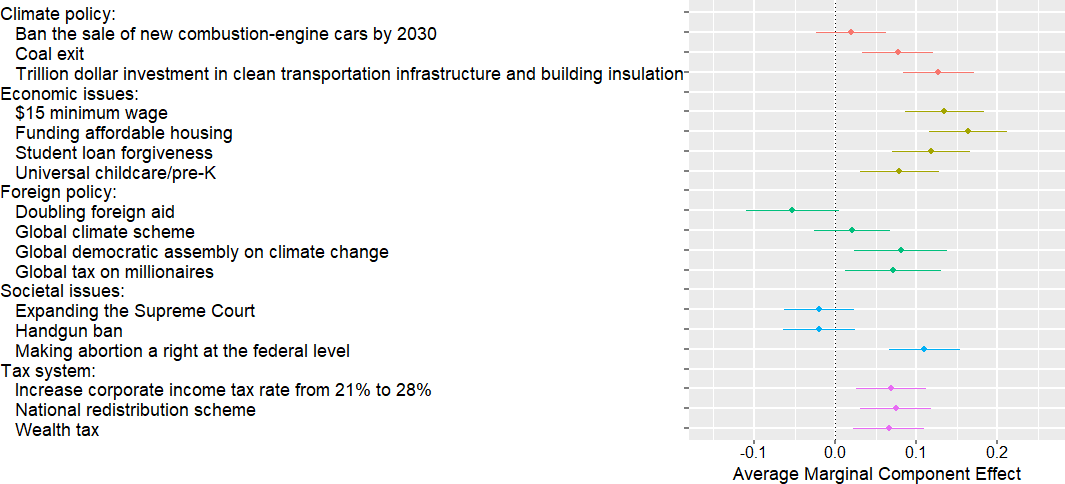
\includegraphics[width=\textwidth]{../figures/US1/ca_r.png}
  \end{subfigure}
  \begin{subfigure}{\textwidth}
    \subcaption{France}
    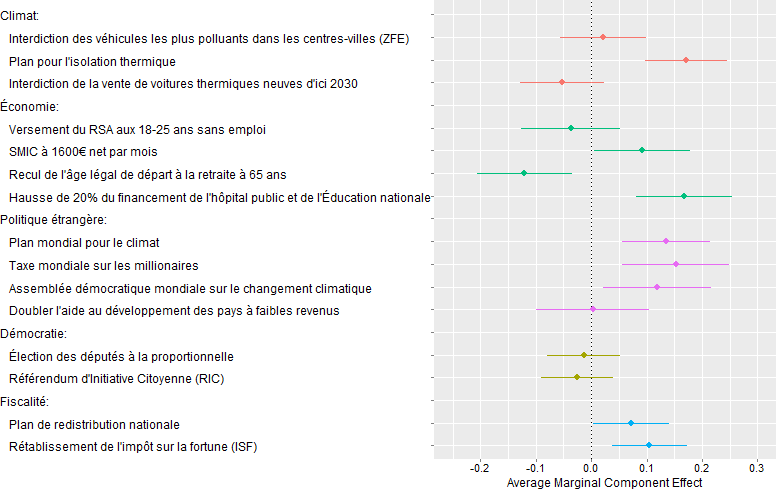
\includegraphics[width=\textwidth]{../figures/FR/ca_r.png}
  \end{subfigure}
\end{figure}%
\clearpage
\begin{figure}[h!]\ContinuedFloat % if bugs try b! instead of h!
  \begin{subfigure}{\textwidth}
    \subcaption{Germany}
    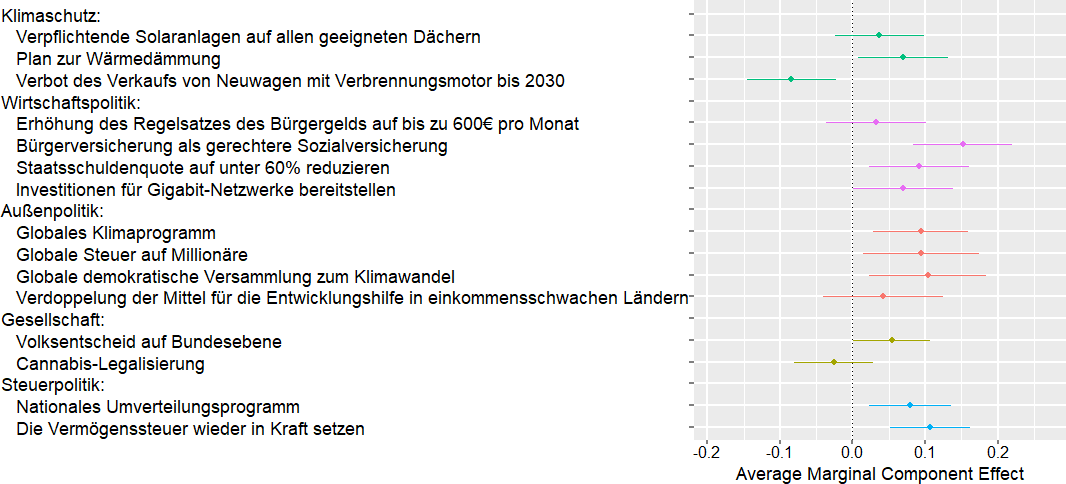
\includegraphics[width=\textwidth]{../figures/DE/ca_r.png}
  \end{subfigure}
  \begin{subfigure}{\textwidth}
    \subcaption{Spain}
    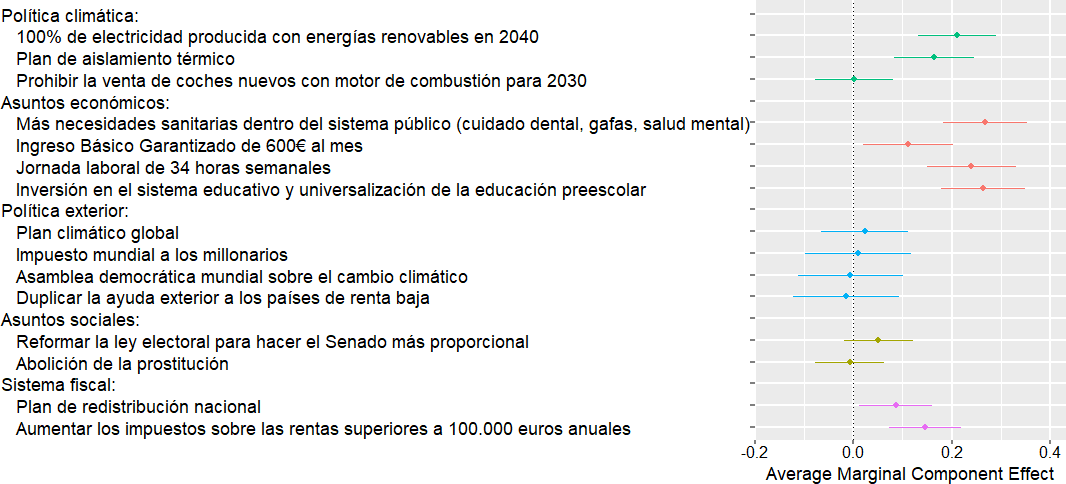
\includegraphics[width=\textwidth]{../figures/ES/ca_r.png}
  \end{subfigure}
  \begin{subfigure}{\textwidth}
    \subcaption{UK}
    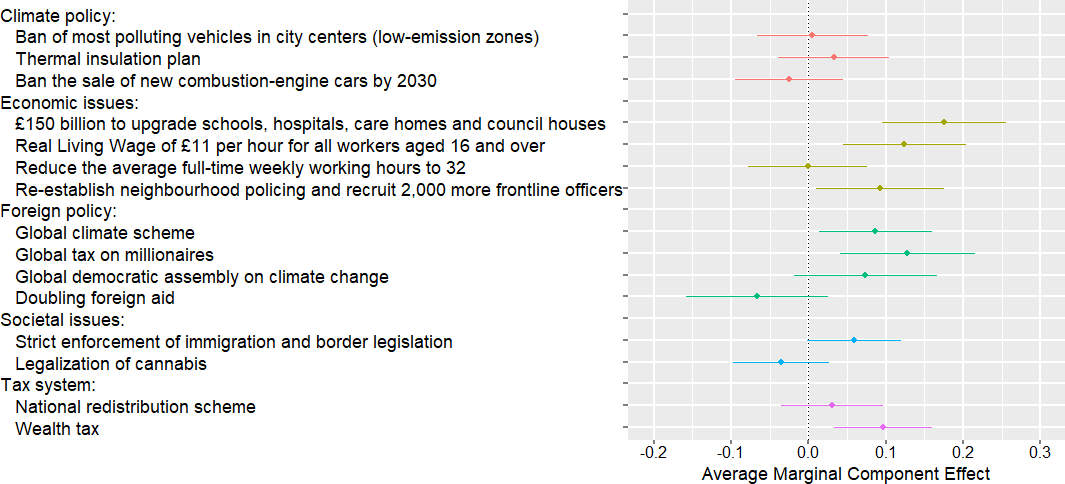
\includegraphics[width=\textwidth]{../figures/UK/ca_r.png}
  \end{subfigure}
  %\makebox[\textwidth][c]{} 
\end{figure}
\clearpage 
\noindent
countries but Spain). 
% Moreover, a platform that includes a global tax on millionaires rather that no foreign policy is 9 to 13 percentage points (p.p.) more likely to be preferred in all countries but Spain (not significant, at +5 p.p.). 
Likewise, a global democratic assembly on climate change has a significant effect of 8 to 12 p.p. in the U.S., Germany, and France. 
%In each country, a platform is more likely to be preferred if it includes the GCS rather than no foreign policy. This effect is significant in France, Germany and the UK, where a platform is about 10 p.p. more likely to be preferred. 
These effects are large, and not far from the effects of the policies most influential on the platforms, which range between 15 and 18 p.p. in most countries (and 27 p.p. in Spain), and all relate to improved public services (in particular healthcare, housing and education). 

The fifth analysis draws random platforms in a similar ways, except that candidate A's platform always contains the GCS while B's includes no foreign policy. In this case, A is chosen by 60\% in Europe %($n$ = 3,000) 
and 58\% in the U.S. (Figure \ref{fig:conjoint_left_ag_b}). %($n$ = 2,218). 
In the U.S. for example, our conjoint analyses indicate that a candidate at the Democratic primary would have more chances to obtain the nomination by endorsing the GCS, and this endorsement would not penalize her or him at the presidential election. This result reminds the finding that 12\% of Germans shift their voting intention from SPD and CDU/CSU to the Greens and the Left when they are told that the latter parties support global democracy \citep{ghassim_who_2020}.

\begin{figure}[h!]
    \caption[Influence of the GCS on preferred platform]{Influence of the GCS on preferred platform:\\ Preference for a random platform A that contains the Global Climate Scheme rather than a platform B that does not (in percent). (Question \ref{q:conjoint_d}; in the U.S., asked only to non-Republicans.)}\label{fig:conjoint_left_ag_b}
    \makebox[\textwidth][c]{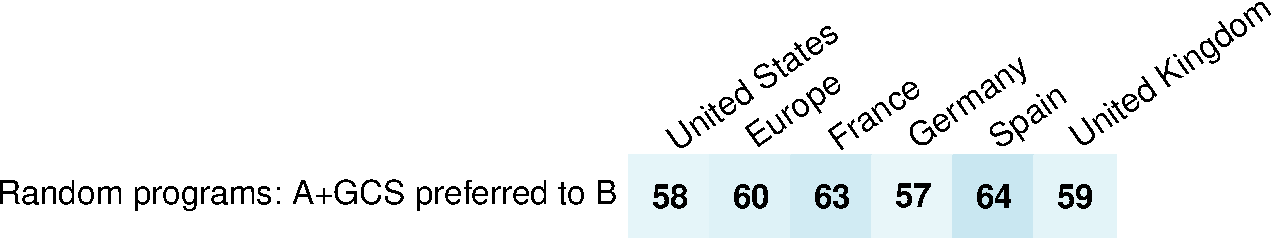
\includegraphics[width=\textwidth]{../figures/country_comparison/conjoint_left_ag_b_binary_positive.pdf}} 
\end{figure}

% \begin{figure}
%   % Imagine that at the 2024 Democratic party presidential primaries, the two main candidates campaign with the following key policies in their platforms. \\ Which of these candidates do you prefer?

%   \caption{Conjoint analysis. Average Marginal Component Effects (relative to the baseline: an absence of policy of that category) of policies in the choice between two platforms, where policies in each platform are randomly drawn ($n$ = 6,000). In Eu, it is framed as two potential platforms of a left-wing coalition that would win the next elections; in the U.S., it is framed as a hypothetical duel in the 2024 Democratic primary and asked only to non-Republicans.}\label{fig:ca_r} % TODO: add ref to Question
%   \makebox[\textwidth][c]{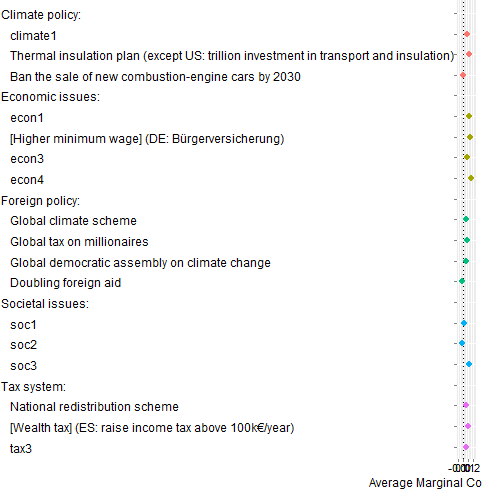
\includegraphics[width=\textwidth]{../figures/all/ca_r.png}}
% \end{figure}

\subsubsection{Prioritization} % Addresses acquiescence bias and social desirability bias
% H1: Prioritization: G has mean only slightly lower than average, makes better than ban of cars and coal exit; global tax on millionaires does as well as wealth tax and almost as good as $15 minimum wage
At the end of the survey, we pick six policies at random (and uniformly) among the policies used in the last conjoint analyses, and ask respondents to allocate 100 points among them (using sliders), with the instruction that ``the more you give points to a policy, the more you support it''. For each policy presented, the average support is thus 16.67 points. %(Figure \ref{fig:points}). % TODO! figures for each country
In each country, the GCS ranks in the middle of all policies or at a higher rank, with an average number of points from 15.4 (U.S.) to 22.9 (Germany). 
In Germany, the the global tax on millionaires is the most prioritized policy and  the GCS the second most. The global tax on millionaires ranks at worst in fifth position (out of 15 or 17) in every country, and receives an average number of points from 18.3 (Spain) to 22.9 (Germany). 
This question further reveals the potential mismatch between policies prioritized by the public and those enacted by legislators. Indeed, to ``ban the sale of new combustion-engine cars by 2030'' is one of the three least prioritized policies in each country, with an average of 7.8 (France) to 11.4 (UK), and yet the European Union and California have enacted to phase out %a target of no 
new combustion-engine cars by 2035. 
%It is higher than to ``ban the sale of new combustion-engine cars by 2030'' (13.4) and ``coal exit'' (10.0), but lower than the third climate policy: ``trillion dollar investment in clean transportation infrastructure and building insulation'' (20.3). The support for other globally redistributive policies is variable: ``Doubling foreign aid'' is the least supported policy (8.4), while the ``Global tax on millionaires'' is one of the five policies with more than 20 points (20.2), and the ``global democratic assembly on climate change'' is just below the GCS (14.5). The most supported policies are ``Funding affordable housing'' (28.5), ``\$15 minimum wage'' (23.8), and ``Universal childcare/pre-K'' (22.1). % TODO? share that allocated at least 1

% \begin{figure}[h!]
%   \caption{Prioritization of policies. Each respondent faces six policies taken at random from the ones below and allocates 100 points among them to signal the strength of their support for each one ($n$ = 3,000).} % Imagine you have 100 points that you can allocate to different policies. The more you give points to a policy, the more you support it.  \\  How do you allocate the points among the following policies?  
  
%   \makebox[\textwidth][c]{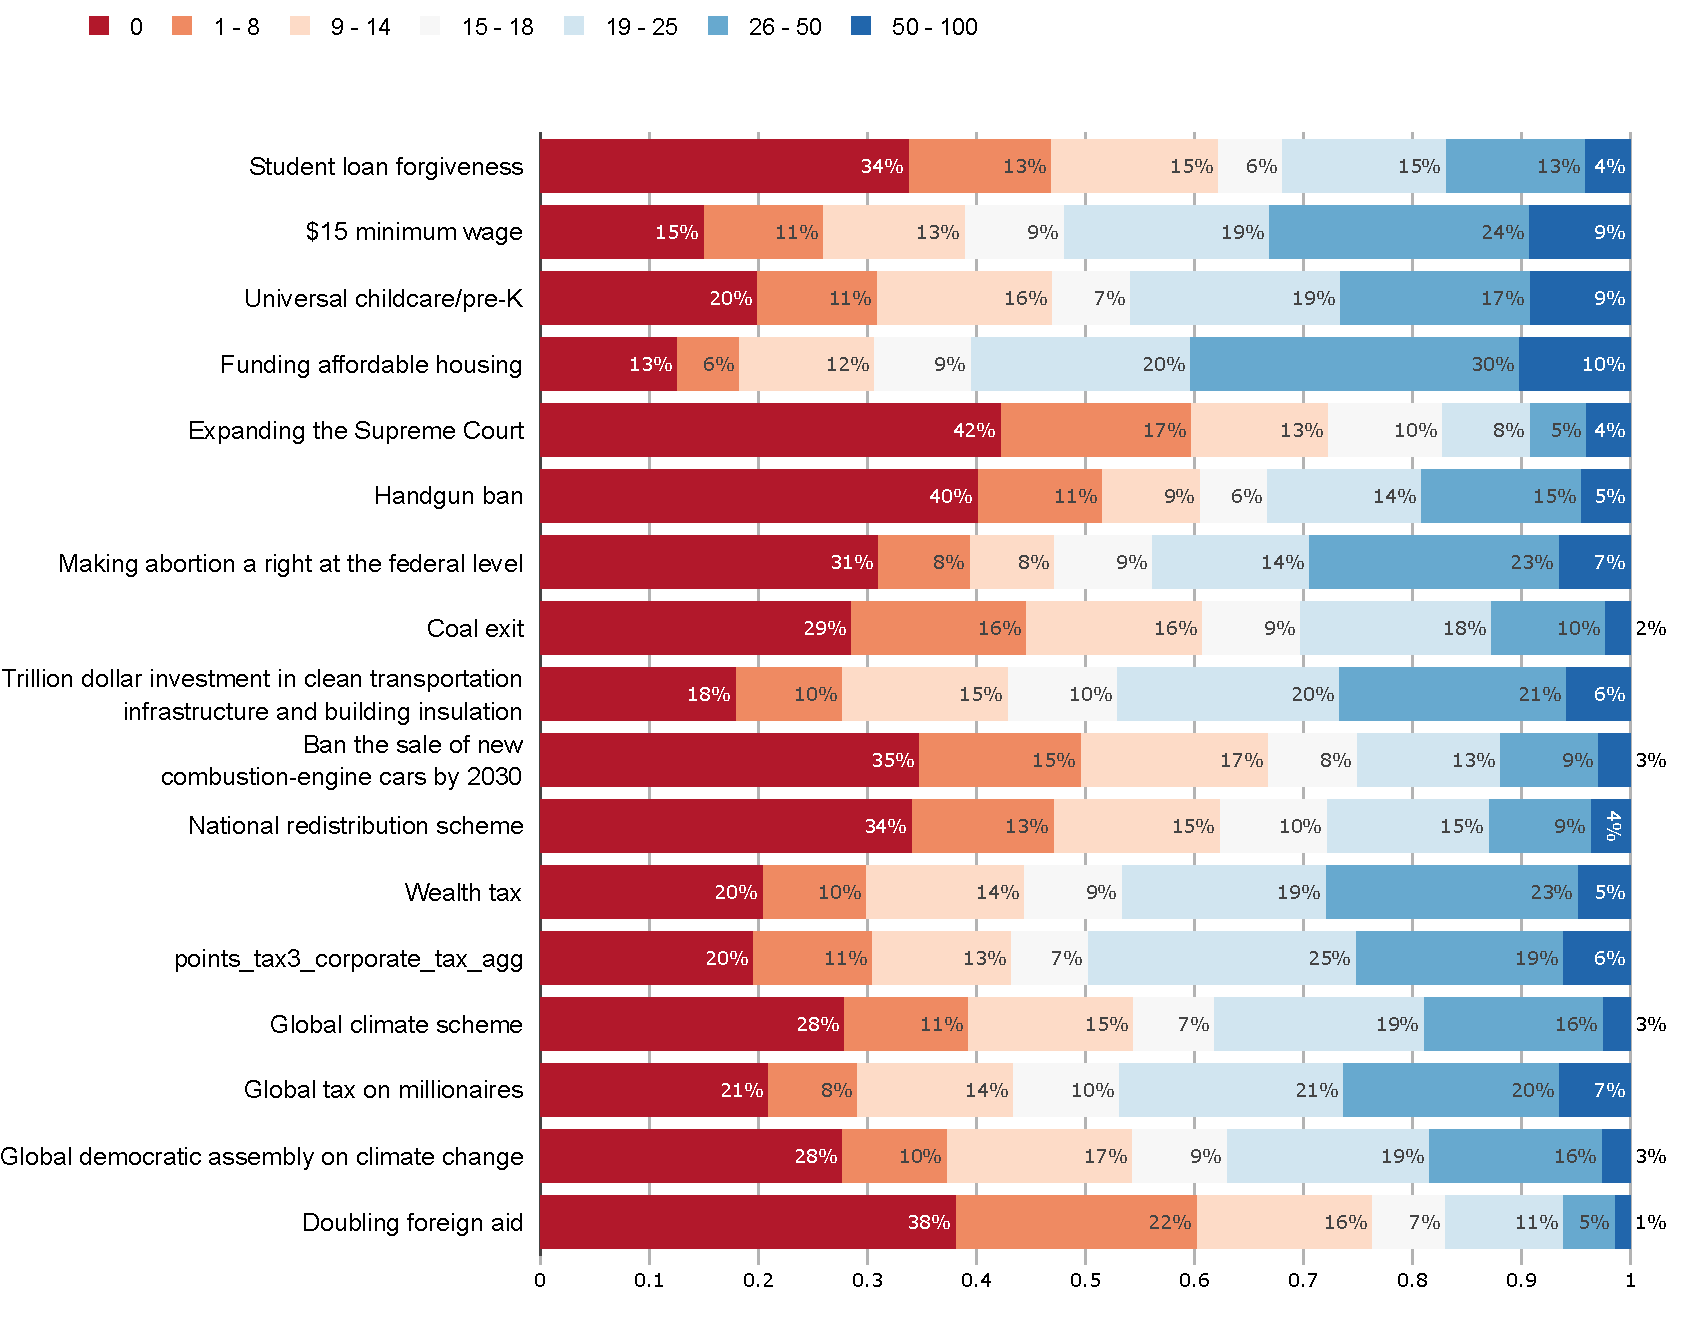
\includegraphics[width=\textwidth]{../figures/US1/points_us.pdf}}\label{fig:points}
% \end{figure}


\subsection{Second-order beliefs}
% H3 belief: No pluralistic ignorance
To explain a strong support for the GCS despite its absence from political platforms and the public debate, we hypothesized pluralistic ignorance, i.e. that most people and policy-makers wrongly perceive the GCS as unpopular. People would then hide their support for such globally redistributive policies, knowing that advocating for them would be vain. We find limited evidence for pluralistic ignorance in an incentivized question on the perceived support (Figure \ref{fig:belief}). Americans have quite accurate beliefs regarding the level of support for the GCS. Indeed, the mean (resp. quartiles) perceived support is 52\% (resp. 36\%, 52\%, 68\%%, $n$ = 3,000
) vs. an actual support of 53\%. Europeans underestimate the support by 17 p.p., but 65\% of them correctly guess that the GCS obtains a majority (mean of 59\% and quartiles of 43\%, 61\%, 74\% vs. an actual support of 76\%). For the record, the second-order beliefs are equally accurate for the National Redistribution Scheme in the U.S., and equally underestimated in Europe.%, with mean (resp. quartiles) perceived support of 54.7\% (resp. 40, 55, 71\%, $n$ = 3,000) vs. 56\%.

\begin{figure}[h!]
    \caption[Beliefs about support for the GCS and NR]{Beliefs regarding the support for the GCS and NR. (Questions \ref{q:gcs_belief} and \ref{q:nr_belief})}\label{fig:belief}
    \makebox[\textwidth][c]{
\includegraphics[width=.7\textwidth]{../figures/country_comparison/belief_all_mean.pdf}} 
\end{figure}

\subsection{Pros and cons}
We ask respondents what are the pros and cons of the GCS, either in an open-ended or in a closed question. In the closed question, people tend to find every argument presented as important to determine their support or opposition to the GCS (Figure \ref{fig:gcs_important}). The least important element is that the GCS ``would penalize my household'' (60\% find this important in Europe -- $n$=1,505, 75\% in the U.S. -- $n$=493). The most important elements differ in both regions: in Europe, it is that the GCS ``would succeed in limiting climate change'' and ``would reduce poverty in low-income countries'' (85\% each) while in the U.S., it is ``having enough information on this scheme'' (89\%) followed by ``it could foster global cooperation'' (82\%). Given the small variation in the importance of each element, the closed question is not very informative. % TODO? distinguish between supporters and opponents?

The open-ended question gives interesting insight into ``what comes to [people's] mind'' when ``thinking of the GCS''. Searching for keywords in the fields (automatically translated into English), the topics that appear most frequently are the international aspect and the environment (each in about one quarter of answers, see Figure \ref{fig:gcs_field_contains}), followed by the effects on poverty and on prices (about one tenth each). We also classified manually each answer into different categories (Figure \ref{fig:gcs_field}). This exercise confirms the automatic search: the most frequent topic is the environmental benefit of the GCS, while the obstacles to implement it or to get %people or countries 
agreement on it are relatively seldom mentioned.\footnote{Besides, one in four people explicitly cite a pro or a con. Few people express explicitly their support or opposition, or exhibit a misunderstanding. Only 11\% of answers are empty or express a lack of opinion, though one quarter are unclassifiable (either because the idea they convey is rare or because it is nonsensical or out of topic).} % TODO n

In the US2 survey, we displayed these questions only to random subsamples, \textit{before} asking for the support to the GCS or NR. The sample was divided into four branches: two with questions on pros and cons (either in closed or open form), one with information on the actual level of support for the GCS and NR (estimated in US1), and one control (without these questions).\footnote{Consistent with Americans correctly perceiving the levels of support for the GCS or NR, providing information on the actual level has no substantial effect on their support. In the closed question on pros and cons, we deliberately included more cons (6) than pros (3) to conservatively estimate what could be the campaign effect on the GCS, i.e. the shift in opinion due to media coverage of the proposal. The campaign effect could play a role, as the support for the GCS decreases by 11 p.p. after people see a list of its pros and cons% (Table \ref{tab:branch_gcs})
. More surprisingly, the support for National Redistribution also decreases (by 7 p.p.) after the closed question on the GCS. This suggests that some people may lack attention and confuse the two policies, or that pondering pros and cons changes the mood of some people, away from a positive first impression. Indeed, the support also decreases, by 7 p.p., after people are asked to think about its pros and cons in an open-ended question.} Despite some significant effects of pondering pros and cons(Table \ref{tab:branch_gcs}), about half of Americans support the GCS in all treatment branches. To the extent that effects would be similar in Europe, this suggests that the GCS would still obtain strong majority support among Europeans after it enters the public debate. 


\subsection{Universalistic values}
% H4: A strong majority is universalist/cosmopolitan (TODO: which word?), even a majority for non-Republican
% TD It is not obvious how these answers are informative of malleable opinions. So I don't think we should state the hypothesis and sell this as a test.
%Another hypothesis to explain the discrepancy between the lack of interest for global policies in the public debate despite a strong stated support is that opinions on the topic are weak and malleable. A way to test this is to
We ask broad questions on people's values to see whether their core values are consistent with universalism. When asked what group they defend when they vote% ($n$ = 6,000)
, 20\% choose ``sentient beings (humans and animals)'', 22\% ``humans'', 33\% their fellow citizens (or ``Europeans''), 15\% ``My family and myself'', and the rest (10\%) choose another group (mostly ``My State or region'' or ``People sharing my culture or religion''). The first two categories can be described as universalist, and they represent close to one out of two people. The share of universalist even constitutes a majority of left-wing voters. % TODO check
When asked what should their country's diplomats defend in international climate negotiations, only 11\% prefer their country's ``interests, even if it goes against global justice''; 30\% prefer global justice (mitigated or not by national interests) and the bulk of respondents (38\%) prefer their country's ``interests, to the extent it respects global justice''. % ($n$ = 6,000). 
Furthermore, when asked to judge the extent to which climate change, global poverty, and inequality in their country are an issue, climate change is generally viewed as the biggest problem (with a mean of 0.59 once we recode answers between $-2$ and $2$), followed by global poverty (0.42) and national inequality (0.37). %, $n$ = 6,000). 

Finally, we elicit unversalistic values through a lottery experiment. We automatically enroll the respondents in a lottery with one \$100 prize. Respondents have to choose which share of the prize to keep for themself vs. give to a person living in poverty. The charity donation is destined either for an African or a fellow citizen, depending on the respondent's random branch. We observe no significant variation in the willingness to donate in function of the recipient's origin in Europe, and a donation lower by 3 p.p. for the African in the U.S. (the average donation is 34\%). Moreover, the slightly lower donations to Africans are entirely driven by right-wing voters or non-voters. 

Overall, answers to these broad value questions are consistent with half of Americans and three quarters of Europeans supporting global policies like the GCS: people are almost as much willing to give to poor Africans than to poor fellow citizens, find that global issues are among the biggest problems, almost half of them are universalist when they vote, and most of them wish that their diplomats take into account global justice.
